% chktex-file 10
\documentclass[a4paper, 12pt]{article}

% include required packages
\usepackage[T1]{fontenc}                   % Font encoding for special characters
\usepackage{pmboxdraw}                     % Support for box-drawing characters
\usepackage{booktabs}                      % For better table formatting
\usepackage{enumitem}                      % For customizing lists
\usepackage{float}                         % For [H] table placement
\usepackage[a4paper, margin=2cm]{geometry} % Set page margins
\usepackage{indentfirst}                   % Indent first paragraph of sections
\usepackage[utf8]{inputenc}                % UTF-8 input encoding
\usepackage{listings}                      % For code listings
\usepackage[round,authoryear]{natbib}      % For citations
\usepackage{tikz}                          % For drawing diagrams
\usepackage{titling}                       % For customizing title
\usepackage[hyphens]{url}                  % For formatting URLs with hyphen breaks
\usepackage{verbatim}                      % For including verbatim files
\usepackage{xcolor}                        % For colors
\usepackage{array}                         % For advanced table column formatting
\usetikzlibrary{positioning, shapes.geometric}               % For relative positioning and diamond node shape

% Allow URLs to break at more characters
\def\UrlBreaks{\do\/\do-\do_}

% set paragraph and list formatting
\setlength{\parindent}{1.5em}
\setlength{\parskip}{0pt}
\setlist[itemize]{noitemsep,topsep=0pt,parsep=0pt,partopsep=0pt,after=\vspace{0.5em}}

% set title information
\title{A critical reflection on refactoring the Web Witchcraft and Wizardry project}
\posttitle{\par\end{center}
    \begin{center}
    \large\url{https://witches-and-wizards.edmundmulligan.name}
    \end{center}
    \vskip 0.5em
}
\author{Edmund Mulligan}
\date{\today}

% Configure listings for JSON
\lstdefinelanguage{json}{
    basicstyle=\small\ttfamily,
    numbers=left,
    numberstyle=\tiny,
    stepnumber=5,
    numbersep=8pt,
    showstringspaces=false,
    breaklines=true,
    frame=lines,
    backgroundcolor=\color{gray!10},
}

% document start
\begin{document}

% set bibliography style and page numbering
\bibliographystyle{plainnat}
\pagenumbering{arabic}

\maketitle

\begin{abstract}
\textit{This is a personal reflection on the design and implementation of a refactored version of a
website.\@ The new architecture is described, along with the navigation design, responsive and
accessibility features, testing strategy, known issues and future improvements. Third party
credits and resources are also acknowledged.}
\end{abstract}

\section{Introduction}\label{sec:introduction}

Web Witchcraft and Wizardry \citep{mulligan2024witchcraftandwizardry} is a website for children  
to learn the basics of web development through fantasy-themed metaphors. The original version of 
the website was neither accessible (except by accident) nor responsive. This essay reflects on the 
design and implementation of a refactored version of the project, focusing on architecture, 
accessibility and code quality. Detailed decisions are documented as comments in 
the source code (available on the \texttt{main} branch at 
\url{https://github.com/Birkbeck2/puffin-web-development-website-edmundmulligan}), so this essay 
focuses on higher level design decisions and reflections.

For comparison the old and new landing pages can be seen in 
figures~\ref{fig:old-landing-page},~\ref{fig:new-landing-page-computer} 
and~\ref{fig:new-landing-page-mobile}.

\begin{figure}[H]
    \centering
    \includegraphics[width=0.8\textwidth]{screenshots/Original Website.png}
    \caption{Old landing page}\label{fig:old-landing-page}
\end{figure}

    \begin{figure}[H]
        \centering
        \includegraphics[width=0.8\textwidth]{screenshots/New-Landing-Page-Computer.png}
        \caption{New landing page on a computer}\label{fig:new-landing-page-computer}
\end{figure}

\begin{figure}[H]
    \centering
    \includegraphics[width=0.3\textwidth]{screenshots/New-Landing-Page-Mobile.png}
    \caption{New landing page on a mobile device}\label{fig:new-landing-page-mobile}
\end{figure}

The development process used was iterative and incremental \citep{beck2004extreme}, and 
while there are criticisms of this approach, particularly around its lack of documentation, 
endless changes and lack of scalability to large teams (see, for example, \citealt{boehm2004balancing}), 
it was well suited to this small project. The
advantage of being able to make quick changes and see immediate results (especially valuable when
learning new techniques) was to some extent offset by the extra work required to frequently 
refactor code to maintain quality and consistency. The process is informally summarised in 
figure~\ref{fig:dev-process-flowchart}. 
\begin{figure}[H]
    \centering
    % Add 'shapes.geometric' to the TikZ libraries for diamond node support
    \usetikzlibrary{positioning, shapes.geometric}

    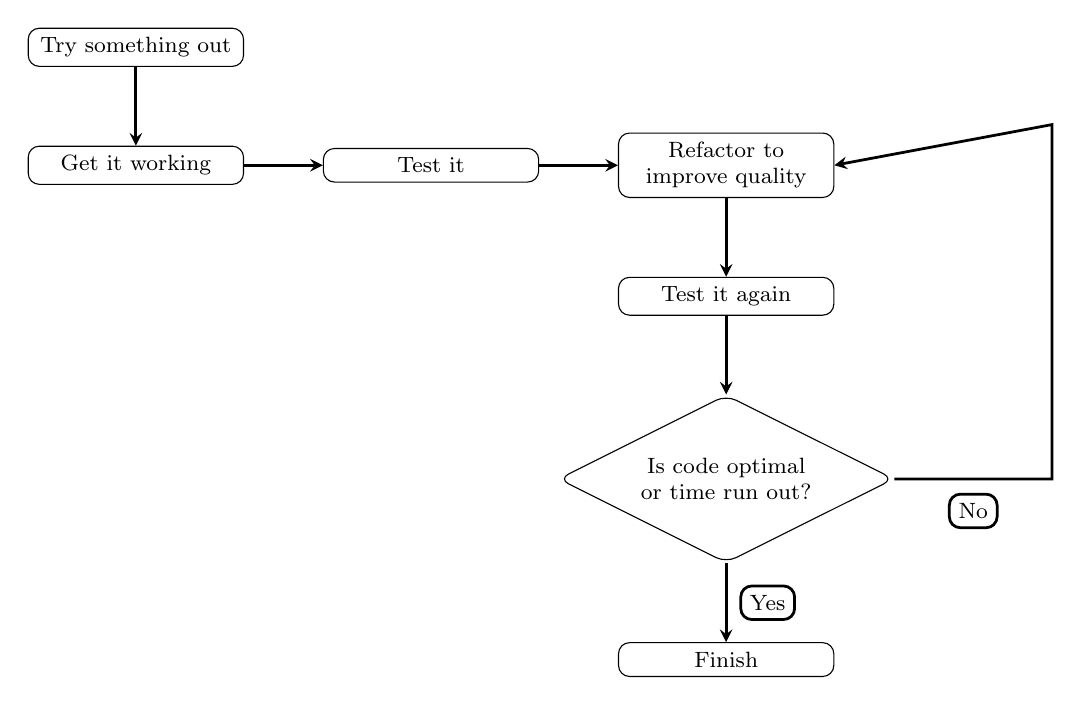
\begin{tikzpicture}
        [node 
            distance=2cm, 
            every node/.style={draw, rectangle, align=center, rounded corners, font=\footnotesize}, 
            ->, 
            >=stealth
        ]
        \node (try) [draw, rectangle, align=center, minimum width=2.5cm, text width=2.5cm] {Try something out};
        \node (work) [draw, rectangle, align=center, minimum width=2.5cm, text width=2.5cm, below=1cm of try] {Get it working};
        \node (test1) [draw, rectangle, align=center, minimum width=2.5cm, text width=2.5cm, right=1cm of work] {Test it};
        \node (refactor) [draw, rectangle, align=center, minimum width=2.5cm, text width=2.5cm, right=1cm of test1] {Refactor to improve quality};
        \node (test2) [draw, rectangle, align=center, minimum width=2.5cm, text width=2.5cm, below=1cm of refactor] {Test it again};
        \node[draw, diamond, align=center, aspect=2, minimum width=2.5cm, text width=2.5cm, below=1cm of test2] (check) {Is code optimal\\ or time run out?};
        \node (finish) [draw, rectangle, align=center, minimum width=2.5cm, text width=2.5cm, below=1cm of check] {Finish};
        \draw[->, >=stealth, line width=1pt] (try) -- (work);
        \draw[->, >=stealth, line width=1pt] (work) -- (test1);
        \draw[->, >=stealth, line width=1pt] (test1) -- (refactor);
        \draw[->, >=stealth, line width=1pt] (refactor) -- (test2);
        \draw[->, >=stealth, line width=1pt] (test2) -- (check);
        % Arrow from east of diamond horizontally 2cm, up 4cm, left 4cm, then down to refactor box north, labeled 'No'
        \draw[->, >=stealth, line width=1pt] (check.east) -- ++(2cm,0) node[midway, below=5pt]{No} -- ++(0,4.5cm) -- (refactor.east);
        \draw[->, >=stealth, line width=1pt] (check) -- node[midway, xshift=1.5em]{Yes} (finish);
    \end{tikzpicture}
    \caption{Iterative development process flowchart}\label{fig:dev-process-flowchart}
\end{figure}

\section{Architecture}\label{sec:architecture}
Even in a small project, software design principles are important to keep the code 
maintainable
 \citep{gamma1994design}. The three main principles applied in this project were 
separation of concerns \citep{parnas1972criteria}, DRY (Don't Repeat Yourself) 
\citep{hunt1999pragmatic}, and self-documenting code \citep{martin2008clean}.
The first principle lead to the folder structure shown in 
figure~\ref{fig:directory-structure}. One advantage of this is that finding and fixing 
bugs is much easier in well structured code.

The second principle influenced the use of JavaScript to inject common elements into each page 
at runtime, rather than duplicating the code in each HTML file. This also inspired the 
use of CSS variables to define common colours and other styles in one place, rather than
duplicating these values throughout the CSS files.

The third principle required meaningful names and comments and a consistent naming 
convention was used throughout.

A fourth (informal) principle is Keep the CSS as simple as possible and make use of 
cascading styles. 
This is something experienced web developers know and if I were to redo this project I 
would put much more effort into writing simple CSS first time rather than trying to refactor 
complex CSS later. The student.html page is a particular example where the CSS is more complex
than necessary and needs more refactoring but I ran out of time to complete this.

\begin{figure}[H]
    \centering
    \footnotesize
    \begin{verbatim}
root/
├── index.html
├── sitemap.xml
├── sitemap.xls
├── images/
│   ├── (site images)
│   └── fontawesome/
│       └── (svg fontawesome icons)
├── pages/
│   ├── about.html
│   ├── glossary-and-faq.html
│   ├── license-and-credits.html
│   └── students.html
├── scripts/
│   └── (injection JavaScript files)
└── styles/
    ├── index.css
    ├── main.css
    ├── media-queries.css
    ├── media-query-index.css
    ├── pages.css
    ├── noscript.css
    ├── students.css
    └── components/
        ├── buttons.css
        ├── header-and-footer.css
        ├── navigation.css
        └── titles.css
    \end{verbatim}
    \caption{Directory structure of the project}\label{fig:directory-structure}
\end{figure}

\section{Navigation}\label{sec:navigation}
Navigation design was kept simple with a top navigation bar for site-wide navigation 
(figure~\ref{fig:site-navigation}) and an in-page navigation bar for navigating 
within all pages except the landing page (e.g.~figure~\ref{fig:in-page-navigation}, 
although each page is slightly different). Incidentally, the wizard and witch in the 
site header are informally known to the development team as `Joe' and `Helena' respectively.

\begin{figure}[H]
    \centering
    \includegraphics[width=0.8\textwidth]{screenshots/site-navigation.png}
    \caption{Site navigation bar structure}\label{fig:site-navigation}
\end{figure}

\begin{figure}[H]
    \centering
    \includegraphics[width=0.8\textwidth]{screenshots/in-page-navigation.png}
    \caption{In-page navigation bar structure}\label{fig:in-page-navigation}
\end{figure}  

\section{A Responsive and Accessible Website}\label{sec:responsive-accessible}
The main goal of the refactor was to make the website responsive and accessible.
The primary techniques used to achieve responsiveness are media queries and
flexible layouts \citep{marcotte2010responsive}. Accessibility features were 
mainly implemented by ensuring the code conformed to web standards, 
\citep{caldwell2024}, but also by following best practices in the 
HTML markup, such as using semantic and landmark HTML elements \citep{w3c_html5},

\subsection{Using and avoiding media queries}\label{subsec:media-queries}
A point made in several YouTube videos (credited in section~\ref{sec:third-party-credits}) 
is that while media queries are important, they should not be overused. The main 
layout should be flexible enough to adapt to a wide range of viewport sizes 
without the need for frequent breakpoints. Exactly which breakpoints to use is 
a matter of experience (which I lack) and judgement (which I possess in abundance), 
and I eventually settled on standardised breakpoints across 
all pages listed in table~\ref{tab:viewport-breakpoints}.

\begin{table}[H]
\centering
\begin{tabular}{llp{6cm}}
\toprule
	\textbf{Viewport width} & \textbf{Layout} & \textbf{Impact}\\
\midrule
0px to 199px & Very small & Warn users but make best effort to display contents reasonably \\
200px to 799px & Mobile layout & Prefer vertical stacking \\
800px to 1199px & Desktop layout & Prefer horizontal layout \\
1200px and above & Large desktop layout & Take advantage of wider screen \\
\bottomrule
\end{tabular}
\caption{Viewport width breakpoints}\label{tab:viewport-breakpoints}
\end{table}

In order to minimise the use of media queries, I used the \texttt{clamp()} CSS function 
to define fluid typography. A limitation of this is that if the middle value of 
\texttt{clamp()} is defined using a viewport width unit (vw), then the text will 
not scale if the user zooms their browser without changing the viewport window size. 
This contravenes WCAG 2.2 Success Criterion 1.4.4 \citep{caldwell2024} which 
requires text to be resizable up to 200\% without loss of content or 
functionality. The workaround for this is to calculate the 
middle value of \texttt{clamp()} from a vw unit and a rem unit, so that zooming 
the browser window also changes the text size.

One downside of this approach is that it takes a lot of trial and error
to find suitable values to pass to \texttt{clamp()} that work well across a wide range of
viewport sizes and this took up much of my testing time. The process was made 
a lot easier when I discovered, at a late stage, an online tool to help calculate 
fluid typography values \citep{bece2025}. 

\subsection{Flexbox vs Grid}\label{subsec:flexbox-vs-grid}
One of the debates I encountered in many tutorials was whether to use CSS Flexbox
\citep{w3c_flexbox} or CSS Grid \citep{w3c_grid} for layout. 
My conclusion was to use flexbox in narrower viewports as this could make vertical 
stacking of elements easier with 
\texttt{flex-direction: column}, and to prefer flexbox with \texttt{flex-direction: row} in wider 
viewports unless there was an obvious case for a grid such as the input form on the 
student page and the gallery of portraits. Due to my experimental approach to 
development, early versions of the website had several levels of nested grids and 
flexboxes which then had to be refactored to simpler layouts later. I also evetually 
realised that flexbox for vertical stacking is not always necessary as block elements 
naturally stack vertically. This is another area where more experience would have helped 
in making better design decisions earlier in the development process.

\subsection{Units of measurement}\label{subsec:units}
Another way to achieve responsiveness is to use relative units of measurement
rather than absolute units. Thus, I used \texttt{rem} units for specifying element sizes. 
I avoided using \texttt{px} units except in media queries where absolute measurements 
are required. I preferred \texttt{rem} units over \texttt{em} units as rems are relative to the root 
font size, making them more predictable, whereas ems are relative to the font size of
the parent element, which can (and did) lead to unexpected results.

\subsection{Browser compatibility}\label{subsec:browser-compatibility}
Ensuring browser compatibility is an important part of web development, 
particularly when using newer CSS features that may not be supported in all browsers.
I used caniuse.com \citep{caniuse2025} and only used HTML/CSS features that were 
supported by all major browsers (Chrome, Firefox, Safari and Edge). One feature I 
particularly wanted to try was \texttt{popover} to avoid having to use JavaScript \texttt{alert()}. 
I was mostly successful but could not get it to work with the form submit button 
(in student.html) so the Save Information button currently does nothing when 
clicked. That will be resolved with JavaScript in phase 2 of the project.

On a related note, all file pathes were specified as absolute rather than relative. 
This is not best practice, but it
avoided issues as I moved files around during development and refactoring. 
The website will break if it is not deployed into the root directory of a 
web server, but that is an acceptable limitation for now.

\subsection{Other accessibility features}\label{subsec:other-accessibility}
The accessibility testing tools sometimes flagged issues with ARIA \citep{w3c_aria} 
compliance. I did not have time to fully investigate these issues, but I
incorporated sufficient ARIA features to satisfy the testing tools. This certainly
deserves further investigation in the future.

Choice of colours and contrast is very important, not only to make a site accessible
but also visually appealing. This is another area where I have little design
experience so I defer the aesthetic aspects of colour choice to next term's module,
where that is covered more fully. For this phase of the project, I limited 
myself to ensuring that the colour choices were not too garish and that 
the choices passed the contrast tests in the accessibility tools. The purple and 
cyan colours were chosen as they (approximately) match the Embodied Mind logo used 
in the footer; the yellow and green were more arbitary.

Testing without a mouse and with a screen reader ensured that that the \texttt{:focus} 
pseudo-class was styled appropriately to make it clear which element had focus and 
meaningful alt text was provided for all images. Using the web site in this way
was not particularly pleasant or easy and emphasises how important it is to design for
accessibility from the start to ensure that those who have no choice but to use 
assistive technologies have as good a user experience as can be achieved.

\section{Testing}\label{sec:testing}
Testing software is not only a critical part of development 
(\cite{myers2011art},\cite{mesbah2012invariant}), but it is also difficult and 
time consuming. Many authorities (e.g.~\cite{boehm1981software},~\cite{jones2008applied})
claim that testing can take at least 50\% of total development time, and that concurs with 
my experience.

My approach to testing was to automate as much as possible using
open source tools (see Appendix~\ref{sec:automated-test-results} for results). The tests were designed to check for compliance 
with web standards (as a proxy for accessibility) and (given the age of the target users) text 
readability. Both static and dynamic testing tools \citep{myers2011art} were used \textemdash{} 
static tools to check code validity, and dynamic tools to check accessibility of the rendered pages.

The tests were run frequently during development to catch issues early and ensure that the 
code remained compliant as it was refactored (regression testing). A github action was 
written to ensure the tests were run whenever code was pushed to the remote development and 
main branches in github. Testing tools were discovered using a google search and the most 
popular ones were chosen:

\begin{itemize}
    \item Lighthouse \citep{lighthouse2025}
    \item Axe \citep{axe2025}
    \item Pa11y \citep{pa11y2025}
    \item Wave \citep{wave2025} 
\end{itemize}

A script to check reading age using the Flesch-Kincaid formula 
\citep{flesch1948new} and Gunning Fog index \citep{gunning1952technique} 
was developed using the \texttt{text-readability} node.js module \citep{textreadability2025}. 
Code was checked for validity using node.js modules \texttt{html-validate} \citep{htmlvalidate2025},
\texttt{stylelint} \citep{stylelint2025} and \texttt{eslint} \citep{eslint2025}. The official W3C 
validator for CSS \citep{w3c_css_validator} was not used as this cannot currently validate 
code with CSS variables. Browser compatibility was tested using Playwright \citep{playwright2025} to 
run tests in multiple browsers and I acknowledge, with thanks, the assistance I received to 
get this working from a senior tester colleague at TfL. This allowed automated testing of 
the latest versions of all three major browser engines (Chrome, Firefox and Safari). 
Playwright has potential for much more and could enable a test driven 
development (TDD) \citep{beck2003test} approach in future phases of this project.

Implementing Wave testing was the most difficult as it requires a public URL to test and 
github pages are based on a private repository. Making the github repository public was 
considered and rejected as it could introduce unanticipated security risks so, after 
consultation with testing colleagues, \texttt{ngrok} \citep{ngrok2025} was used to expose the 
localhost to allow Wave tests to complete.

There was insufficient time to fully evaluate the third party tools used and decide which 
was the best for this project, so a `black box' approach was taken without investigating exactly 
what each tool was testing. This did have the benefit that gaps in one tool's coverage
could potentially be caught by one of the other tools, but it did incur a risk that the tools 
could change what they reported without notice. Indeed this occured with Wave during the
development of this project, when it stopped reporting that <h1> was in the <header> rather 
than <main> element. This brought it into line with the other tools, but decreases confidence
 in the reliability of the tools.

Automated testing is not a substitute for manual testing, and the site was also tested manually
on a variety of devices, specifically

\begin{itemize}
    \item A computer with a mouse and keyboard (running Linux Mint)
    \item A computer without using a mouse (to test keyboard navigation)
    \item A computer with a screen reader (Linux Orca)
    \item A touchscreen tablet device without mouse or keyboard (running Android)
    \item A mobile phone (running Android)
\end{itemize}

I did not have access to an iOS device so could not test on Apple hardware, nor did I have 
time to test on non-Linux operating systems. Testing was informal and ad hoc rather than
systematic, and with more time, test scripts would be written to ensure consistent coverage
across all devices. This would be more necessary if more than one developer were involved in
the project to ensure everyone tested the same way.

I did not test the website with JavaScript disabled and I acknowledge this as a limitation
of the current testing, driven by the available time. Testing thus far has mainly been 
verification rather than validation \citep{myers2011art}, \citep{IEEE1990}, but when actual
lessons are implemented user and expert validation from a teacher will be needed to ensure 
the content is age appropriate and pedagogically sound. Security, and performance testing 
will also be needed when student data (tracking lesson progress) are collected. 

\section{Outstanding issues and future improvements}\label{sec:outstanding-issues}
The project submitted for assessment is phase one of a larger project to refactor and
improve the Web Witchcraft and Wizardry website. Some content was deliberately omitted 
from this phase as it will be developed in phase 2 using JavaScript. 
Appendix~\ref{sec:bugs} lists some known issues and areas 
for improvement that could not be addressed within the time constraints of this phase.

\section{Third party credits and resources}\label{sec:third-party-credits}
All code submitted for assessment is my own work. No code has been copied from 
any external sources, such as online tutorials or example code. I have, however, relied 
heavily on three YouTube channels, those of Kevin Powell \citep{powell_youtube}, 
Daily CSS \citep{dailycss_youtube}, and Coding2GO \citep{coding2go_youtube}, for 
guidance on best practices and inspiration.

I made extensive use of Google Search, Google Scholar and Stack Overflow to research 
and troubleshoot specific issues I encountered.

The automation tools used for testing accessibility and performance (Lighthouse, Axe, 
pa11y, Wave) are all open source tools developed by third parties and the scripts used 
to run them were adapted from examples found in their respective documentations and in 
online resources. I was assisted by a colleague at my employer, Transport for London, 
in writing the Playwright tests used for testing browser compatibility.

The original artwork used in the website was created by Rachel Mulligan, a professional 
stained glass artist. I am grateful to her for allowing me to use her work in this 
project. The images used in this iteration are an early version and will be refined 
in future phases.

\section{Conclusion}\label{sec:conclusion}
This has been a challenging and rewarding project. The challenge has not been coding the 
website, as I have 40 years of experience doing that, but in learning a lot of new 
material around modern CSS in a short space of time and applying that in a standards based 
development paradigm. The refactored Web Witchcraft and Wizardry website, while not yet 
complete, is a significant improvement on the original version in terms of accessibility, 
responsiveness and code quality. The use of automated testing has helped ensure that the 
code meets web standards and is accessible to the target audience. There are still some 
outstanding issues and areas for improvement that will be addressed in future phases of 
the project.

% Include word count N.B. Run wordcount.sh to generate wordcount.txt before compiling
\section*{Word count}
Word count: \input{wordcount.txt} words (excluding references)
\\

\bibliography{EdmundLibrary}

% include appendices
\newpage
\appendix
\section*{Appendices}
\section{Known Issues and Workarounds}\label{sec:bugs}
This appendix contains known issues and workarounds.

\begin{table}[H]
\centering
\begin{tabular}{l p{4.5cm} p{4.5cm} p{4cm}}
\toprule
\textbf{Issue Id} & \textbf{Description} & \textbf{Symptoms} & \textbf{Work around} \\
\toprule
1 & Responsive code does not work well at extreme viewport sizes & 
    Text overflows boxes or content does not fill screen properly. & 
    Warning displayed when viewport is too small. \\
\midrule
2 & Font sizes are not optimal & 
    Text is too small or too large on some devices. & 
    Further refinement of clamp~() values is needed. \\
\midrule
3 & The artwork provided by Rachel Mulligan is in JPEG format with a white background. & 
    The picture gallery looks ugly with white boxes around images. & 
    Images need to be edited to have transparent backgrounds (PNG or SVG format). \\
\midrule
4 & student.css is a mess. &
    Doesn't conform to the standards in other css files. &
    More refactoring needed. \\
\midrule
5 & Incomplete functionality. &
    Some features are not implemented yet. &
    Further development required to complete all features. \\ 
\midrule
6 & ARIA compliance is minimal. &
    Some elements lack full ARIA attributes. &
    Invesigatin of ARIA, accessibility audit and improvements needed. \\
\midrule
7 & popovertarget does not work on submit buttons. &
    The popover does not appear when clicking the Save Information button. &
    Use JavaScript to show a popover or alert on form submission. \\
\midrule 
8 & Website does not respect system light/dark mode preference. &
    Website always uses light mode even if system is in dark mode. &
    Use CSS media query prefers-color-scheme to adapt to system preference. \\

\bottomrule

\end{tabular}
\caption{Known issues and workarounds}\label{tab:bugs}
\end{table}

\clearpage
\section{Test Outputs}

This appendix contains the complete test results from the automated test suite. All tests were executed on \today{} and demonstrate compliance with web standards, accessibility guidelines, and readability requirements.

\subsection*{Summary of Test Results}

\begin{table}[H]
\centering
\begin{tabular}{|l|l|r|}
\hline
\textbf{Test Type} & \textbf{Metric} & \textbf{Result} \\
\hline
Code Validation & Files validated & 29 \\
 & HTML errors & 0 \\
 & CSS errors & 0 \\
 & JavaScript errors & 0 \\
\hline
Link Checking & Total links checked & 161 \\
 & Broken links & 0 \\
 & Pages checked & 5 \\
\hline
Axe Accessibility & Total violations & 0 \\
 & Critical issues & 0 \\
 & Serious issues & 0 \\
\hline
Lighthouse & Average score & 100\% \\
 & Pages tested & 5 \\
 & Failed audits & 0 \\
\hline
Pa11y Accessibility & Total errors & 0 \\
 & Total warnings & 0 \\
 & Pages tested & 5 \\
\hline
WAVE Accessibility & Total errors & 0 \\
 & Alerts (non-critical) & 10 \\
 & Pages tested & 5 \\
\hline
Reading Age & Average grade level & 9.1 \\
 & Pages analyzed & 3 \\
 & College-level pages & 0 \\
\hline
Browser Tests & Browsers tested & 3 \\
 & Tests passed & 150 \\
 & Tests failed & 0 \\
\hline
\end{tabular}
\caption{Summary of all automated test results}
\label{tab:test-summary}
\end{table}

\clearpage

\subsection*{Detailed Test Results}

The following sections contain the complete JSON output from each test suite.

\subsubsection*{Code Validation Results}
\lstinputlisting[language=json]{../tests/results/validation-results.json}

\clearpage

\subsubsection*{Broken Links Check Results}
\lstinputlisting[language=json]{../tests/results/broken-links-results.json}

\clearpage

\subsubsection*{Axe Accessibility Results}
\lstinputlisting[language=json]{../tests/results/axe-results.json}

\clearpage

\subsubsection*{Lighthouse Accessibility Results}
\lstinputlisting[language=json]{../tests/results/lighthouse-results.json}

\clearpage

\subsubsection*{Pa11y Accessibility Results}
\lstinputlisting[language=json]{../tests/results/pa11y-results.json}

\clearpage

\subsubsection*{WAVE Accessibility Results}
\lstinputlisting[language=json]{../tests/results/wave-results.json}

\clearpage

\subsubsection*{Reading Age Analysis Results}
\lstinputlisting[language=json]{../tests/results/readability-results.json}

\clearpage

\subsubsection*{Cross-Browser Compatibility Results}
\lstinputlisting[language=json]{../tests/results/browser-results.json}



\end{document}
